\chapter{Conclusions~and~Future~Work}
\label{chap:future} 


\section{Future work}
\subsection{Ensemble training and uncertainty estimation}

There exist a number of uncertainty measures specifically developed for object detection based on Bayesian \gls{NMS} \cite{Harakeh}, test time augmentation {Wei2018} and of particular interest based on ensembles \cite{Le2018}. Some discussion in section--\ref{sec:example_selection}. 

K-fold cross-validation is proposed as a future method to improve data usage. It can be used for ensemble based predictions on new images with uncertainty estimation, unbiased reviewing and machine assisted verification to check for mistakes and improved accuracy in testing by testing against the full dataset.

In conflict with our desire to use high resolution images for annotation clarity, ensembles, example selection, and interface responsiveness would all benefit from use of lower resolution images. More experimentation is necessary to determine the best trade off, which seems likely to depend on the dataset.

\subsection{Domain specific applications, counting wildlife}

One promising application for \gls{VBA} has been to counting wildlife, where the annotation tool has been used for verified counting of Antarctic wildlife. A number of limitations were discovered, such as efficiency issues with the user interface in the presence of very large numbers of object, and the difficulties created by artificial splitting of images. Addressing efficiency is very straightforward, but a way of allowing the user to divide up very large images would seem beneficial.

A number of metrics and image selection heuristics were added to attempt to aid experimentation with time series images. Expanding on these heuristics and providing better methods for exploring and sorting images would be beneficial for studying these kind of images. Adding image level classification would also be useful for sorting and managing datasets, for example discarding images with poor visibility automatically would be possible if discarded images are be labelled and used for learning.

\subsection{Higher level forms of object detection}

\begin{figure*}[h!]
\begin{subfigure}[t]{1.0\linewidth}
  \centering
  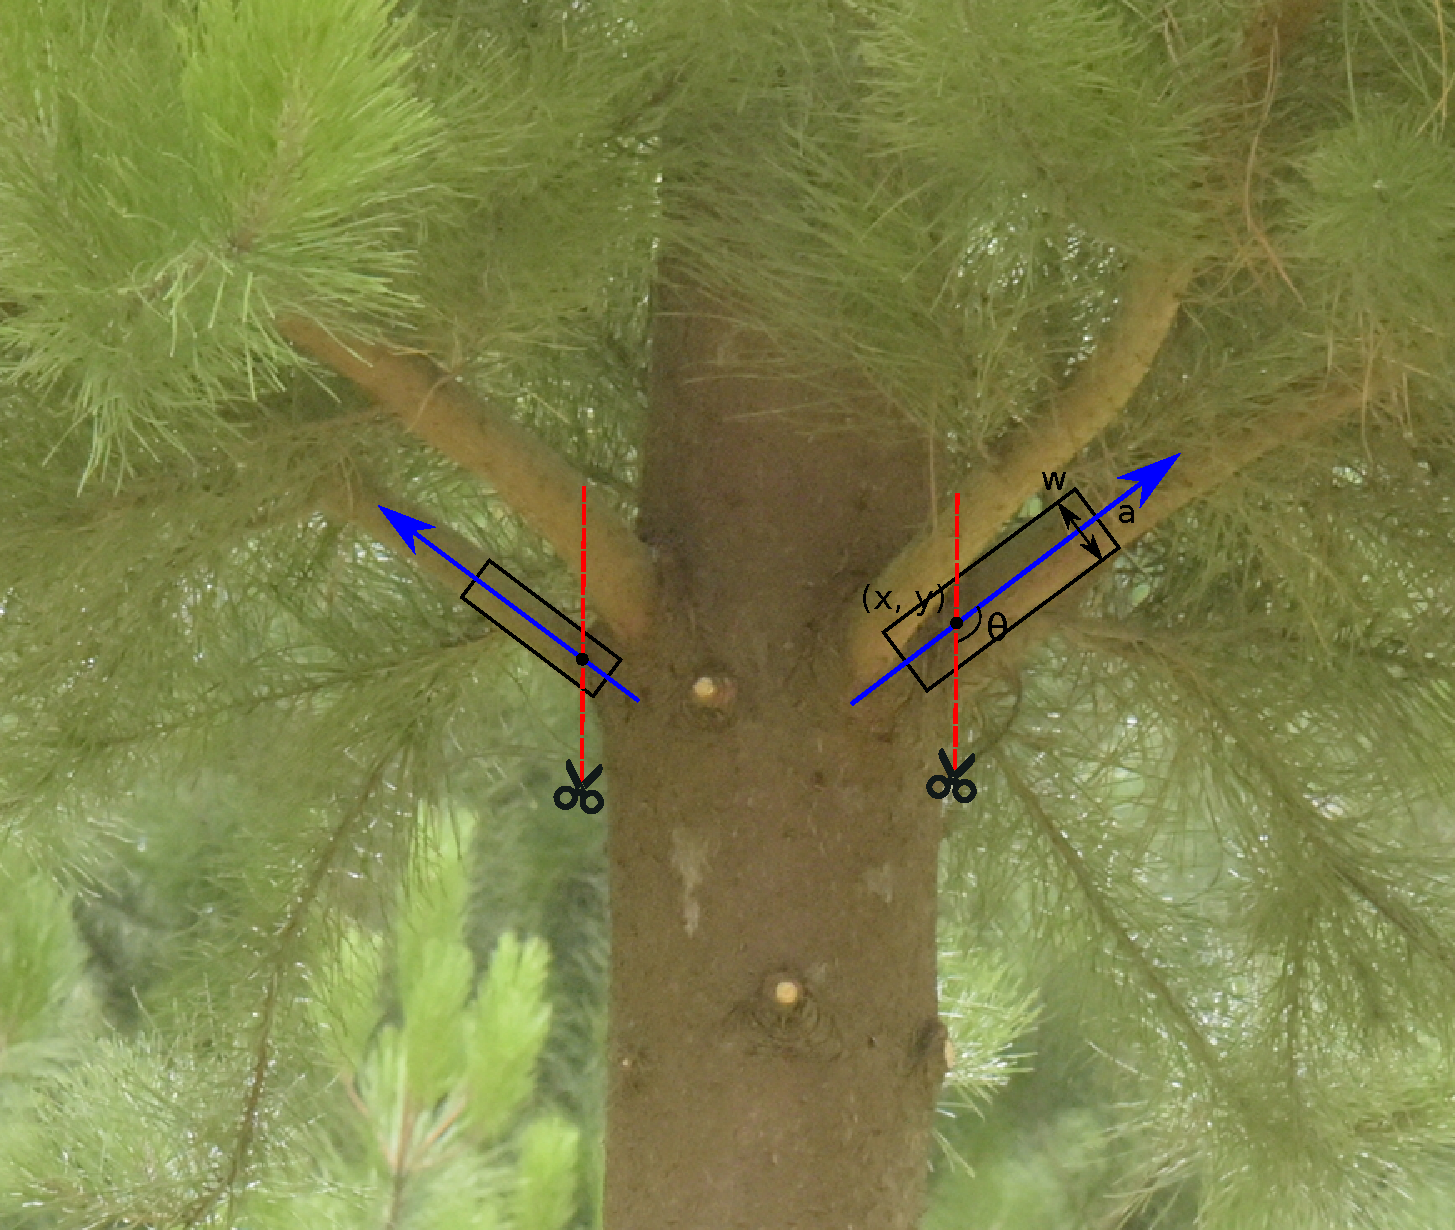
\includegraphics[width=0.8\linewidth]{figures/future/tree_cutpoint.pdf}
  \caption{} 
\end{subfigure}

\begin{subfigure}[t]{1.0\linewidth}
  \centering
  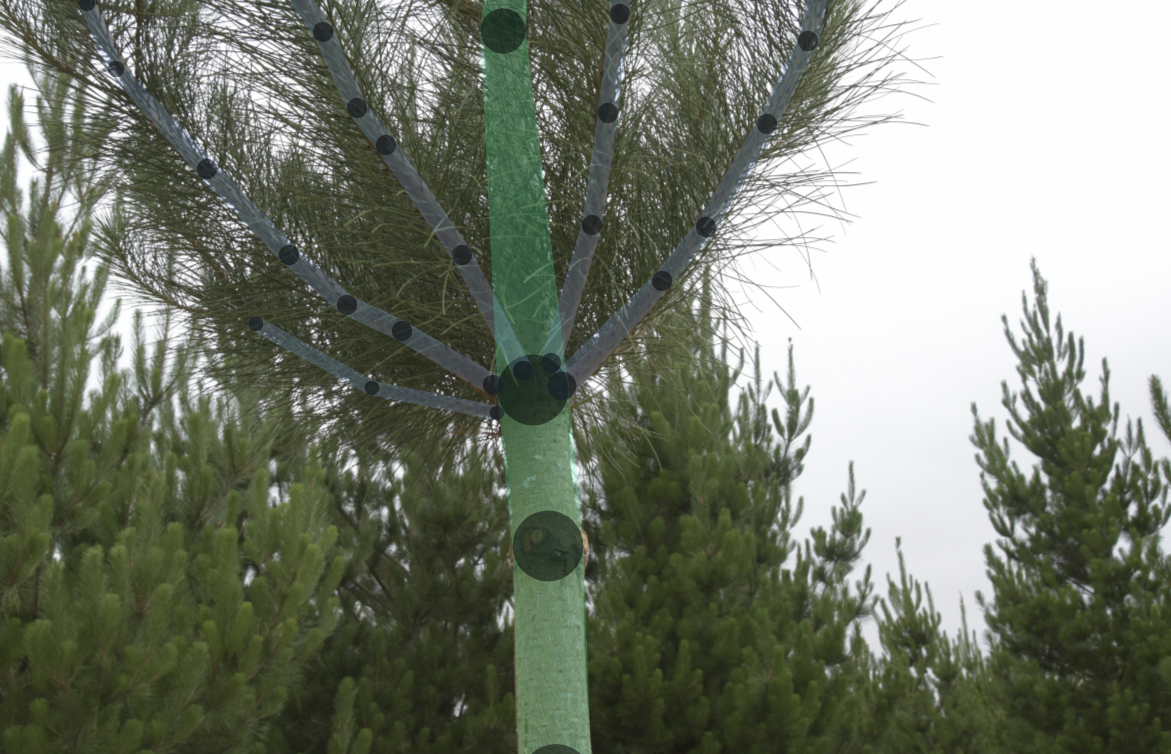
\includegraphics[width=0.8\linewidth]{figures/future/tree_branches.jpg}
  \caption{} 
\end{subfigure}
\caption{Ongoing work into annotating trees in (a) cut-point detection, (b) tree structure skeleton extraction }
\label {fig:future_trees}
\end{figure*}

Bounding boxes have limits for object detection, they only very loosely fit an object. Some objects cannot be described well by bounding boxes at all. Tree branches are fit by bounding boxes very badly; they're very long, and it's not always clear where they start and stop. Future work will focus on other kinds of object detection, and the ability to pick the type for the task at hand.

Recent work in object detection \cite{Zhou2019} or \cite{Law2018}, both successors to the RetinaNet detector \cite{Wang2017} used in this work, have shown that both the anchor box approach, and \gls{NMS} is unnecessary. In \cite{Zhou2019}, local maxima in a single a heat map is used to detect objects, all other parameters are regressed, allowing for simple extension to a range of different types of object detector.

The branches dataset used as an example in this work is a trial for detecting cut positions. Figure~\ref{fig:future_trees} shows two directions in annotation of tree structures, cut point estimation and skeletal extraction for robotic pruning applications. Skeleton estimation on tree structures can be adapted from methods used for road network extraction \cite{Li2018}, shape estimation \cite{Jiang2019a} or polygon extraction \cite{Acuna2018}, and can work well within the \gls{VBA} approach.

One barrier preventing research into new forms of object detection is annotation. Models for detection can be integrated with the verification based annotation approach described in this thesis for experimentation on new forms of object detection.

\subsection{Annotating uncertainty}

In future the ability to annotate images based on uncertainty may be a useful approach, as a means of calibrating confidence and for the purposes of weighting examples in the training process. As opposed to epistemic uncertainty, aleatoric uncertainty can be estimated directly (by a \gls{NN} for example by regression).  

This kind of uncertainty annotation may be also useful in weighting training loss, where the network can place more weight on hard, yet unambiguous examples. The use of Focal Loss means that examples which fail to classify well are weighted much more highly, if these examples are ambiguous because of shadow or lack of resolution - their contribution to the training will be purely as noise.

Hard examples are often cited as being the most useful for an object detector, but if the hard examples are not really hard examples, because they are also visually ambiguous or uncertain (high aleatoric uncertainty) then their usefulness as a learning target might be less, but still possesses value for use in validation and calibration.



\subsection{User verification and testing}
\label{sec:user_verification}

The risk of algorithmic bias brings into the question the quality of a dataset annotated with a \gls{VBA} system.  In order to combat algorithmic bias when a human annotator becomes fatigued, it is proposed that a certain level of \emph{generated} mistakes can be included. Which a user is either forced to fix before they may continue, or is logged as a measure of the user's trustworthiness. For example adding \emph{deliberate} errors into provided detections, such as false positives, false negatives by removing very high confidence detection, or localisation errors by transform box of high confidence detection. 


\subsection{Software improvements}

There are a range of general software improvements to improve usability and prepare for release to a wider audience. Some plans are detailed in chapter~\ref{chap:design}, including: streamlining detection to avoid the need for selecting manual thresholds, simplifying the interface, easy deployment to cloud based systems, integrating and exposing object detection configuration parameters to the user interface and integration of visualisation for metrics.

\section{Conclusion}
\label{sec:conclusion}
\glsresetall

Largely out of frustration with the difficulty of capturing and annotating image data, the goal of this thesis became how to effectively annotate data, in order to apply and experiment with machine learning models on new domains in visual recognition. Specifically, the goal has been to evaluate and characterise the best use of a \emph{human-in-the-loop} annotation method I have termed \gls{VBA}, where a machine learning model is trained interactively based on verifying and correcting predictions from the model. A key point of difference to similar works developed either prior or concurrently to this work is the focus on online training, where existing works largely use either (a) strong models trained on large data sets or (b) staged systems with alternating periods of annotation and training. 

Chapter~\ref{chap:focus} looked at how image cropping effected classification performance using a \gls{CNN}, a prelude to later work which examined annotation noise in object detection. For an instance recognition dataset, it was found that a tight cropping, and increased resolution were both strongly beneficial to classification using a \gls{CNN}.

In chapter~\ref{chap:metric} a novel form of mini-batch deep \gls{NCA} metric learning was presented, using a multi-way comparison between feature vectors. It was surprisingly found to work much better for small batch sizes, and used to learn feature vectors for instance recognition on small images with a \gls{CNN}.

Chapter~\ref{chap:bootstrap} is an exploratory work into different forms of machine assisted segmentation. Several methods were examined using segmentation of tree trunks as a test case. The most promising direction was a method of incrementally training a model while annotating by verifying and correcting machine predictions. Experiments were performed showing that by using fine tuning, surprisingly little data and training time were necessary to achieve workable levels of accuracy to assist annotation. 

Chapter~\ref{chap:design} describes the design and implementation, object detection system on real world data  of a \gls{VBA} system for object detection using lessons learned from chapter~\ref{chap:bootstrap}. A annotation system built around \gls{VBA}, with the option of light active learning was developed, using a web-based interface for easy deployment. I develop a novel method for utilising weak detections, which may be well localised even if not classified correctly was developed (and usage justified in chapter~\ref{chap:annotation}), and a method for using the machine model to aid in reviewing existing annotations was prototyped.

The \gls{CNN} object detector used in the \gls{VBA} annotation tool is described in chapter~\ref{chap:object_detection}. In order to accommodate the needs of online training for image annotation, as opposed to necessarily the strongest or fastest object detector, modifications over standard practice are described, such as avoiding weight sharing, a non normalised loss function, cyclical learning rates and methods for training training and inference using high resolution images developed. Some assumptions were tested, cyclical learning rates were found to have less impact than assumed, methods for training using high resolution images were shown to be both practical and deliver improved accuracy. Finally a study on the effect of noise (introduced by rough annotation) and systematic bias (such as that introduced by algorithmic bias) was examined, showing that for a small amount of bias and human levels noise the object detector is quite robust, but with less data the sensitivity to noise increases greatly and overfitting, thus the annotator should focus on accurate annotation especially at the beginning of the process. 

Chapter~\ref{chap:annotation} presents a series of studies where $10$ different and widely varied image sets were annotated in order to evaluate and explore where the \gls{VBA} system is most applicable. Image sets with a large de  


Future work will focus on several areas (amongst other smaller goals): (a) different forms of object detection, for example polygons, oriented boxes and pose estimation (b) polishing the interface for wider release and easy deployment on cloud services (c) improved use of data, using k-fold cross validation ensembles for uncertainty estimation (d) application to larger scale annotation and multi-user annotation.
